\section{Gateway}
\label{sec:app-gw}

Para a construção do \emph{Gateway} foi feita a instalação e configuração do
\emph{MQTT Broker} \emph{Mosquitto} em um dos RPI3.

\begin{citacao}

	Eclipse Mosquitto™ é um distribuidor de mensagens de código aberto (EPL/EDL
	licenciado) que implementa o protocolo MQTT versões 3.1 e 3.1.1. O MQTT
	fornece um método leve de transmitir mensagens usando um modelo de
	publicação/inscrição. Isso o torna adequado para mensagens "Internet das
	Coisas", como com sensores de baixa potência ou dispositivos móveis, como
	telefones, computadores embutidos ou microcontroladores como o Arduino. \

	\citeonline{mosquitto} Tradução Nossa.
\end{citacao}


A instalação é realizada com o gerenciador de pacotes \emph{apt-get} padrão do
\emph{raspbian} como mostrado na primeira linha da listagem abaixo.

\begin{lstlisting}[language=bash]
pi@broker:~ $ sudo apt-get install mosquitto
pi@broker:~ $ sudo sh -c 'echo "password_file /etc/mosquitto/passwd"
	>> /etc/mosquitto/mosquitto.conf'
pi@broker:~ $ sudo mosquitto_passwd -c /etc/mosquitto/passwd user
Password:
Reenter password:
\end{lstlisting}

Nas linhas 2 e 3 adiciona-se ao arquivo padrão de configuração padrão do
\emph{Mosquitto} a linha 'password\_file /etc/mosquitto/passwd' que
indica o arquivo de senhas a ser utilizado para autenticação. Na linha 4 é
adicionado o usuário 'user' ao arquivo, a senha é solicitada  nas
linhas 5 e 6.

Feito isso o acesso ao \emph{Broker} está limitado aos usuários e senhas
configurados neste processo. As demais configurações permaneceram sem alterações.

Na configuração do sensor deve ser adicionado o endereço (nome ou IP), a porta
\emph{1883} e o par usuário e senha para que este acesse o \emph{Gateway} com
sucesso.

Para verificar o funcionamento do conjunto sensor e distribuidor utiliza-se um
cliente \emph{MQTT} como o aplicativo para \emph{Android} \emph{MQTT Dashboard}
\cite{mqttdash} ou os aplicativos para \emph{Java} \emph{mqtt-spy}
\cite{mqttspy} e para \emph{Windows} \emph{MQTT.fx} \cite{mqttfx}.

Nas figuras \ref{fig-ad-publish}, \ref{fig-ad-home-ack} e \ref{fig-ad-admin-ack}
o aplicativo \emph{MQTT Dashboard} é utilizado para verificar quais sensores
estão online com a mensagem 'echo' publicada no tópico 'ADMIN'. Na
\autoref{fig-ad-publish} os botões enviam mensagens com simplicidade. Na
\autoref{fig-ad-home-ack} é visível a lista de tópicos e a última mensagem
recebida em cada um deles. Na \autoref{fig-ad-admin-ack} fica evidente a
resposta de confirmação (\emph{ack}) de cada um dos sensores.

A aplicação \emph{MQTT.fx}, em especial a tela mostrada na
\autoref{fig-mqttfx-stats}, revela estatísticas do \emph{Broker} como a versão,
tempo \emph{online}, número de clientes, mensagens e utilização de rede.
Na aplicação \emph{mqtt-spy} o comando de listagem mencionado na
\autopageref{code-sensor-mqtt} é demonstrado.

\begin{figure}[htb]
\centering
	\begin{minipage}{0.32\textwidth}
	\centering
		\caption{\label{fig-ad-publish}MQTT Dashboard: Envio de mensagens}
		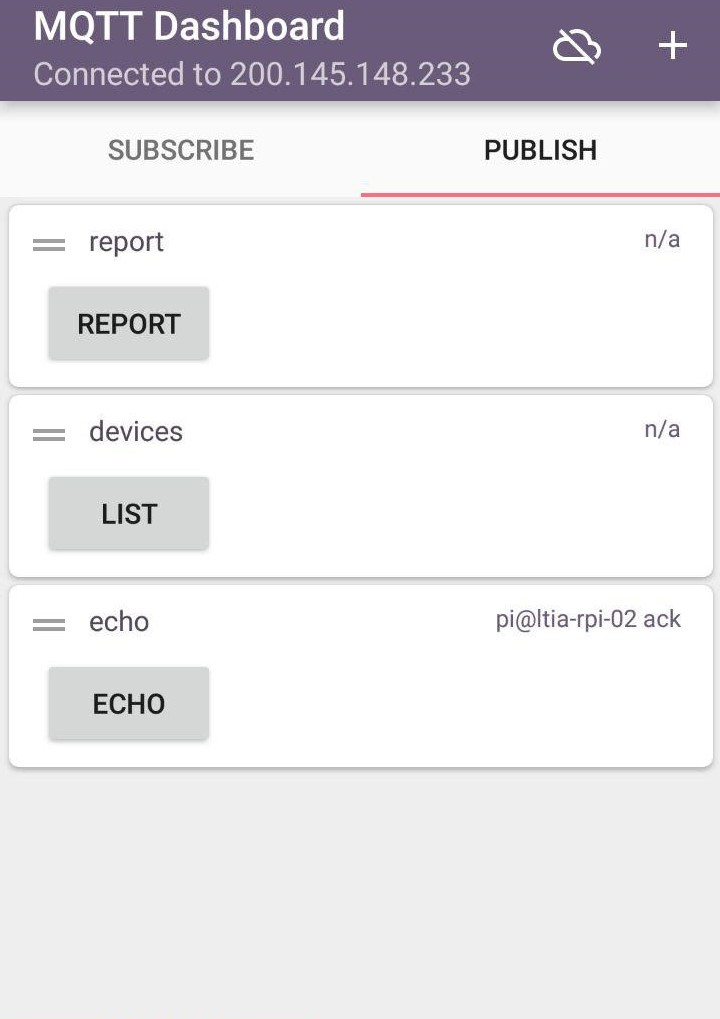
\includegraphics[width=1\textwidth]{052-gateway/mqtt/ad-publish.jpg}
		\legend{Fonte: Produzido pelo autor}
	\end{minipage}
\hfill
	\begin{minipage}{0.32\textwidth}
	\centering
		\caption{\label{fig-ad-home-ack}MQTT Dashboard: Lista de inscrições}
		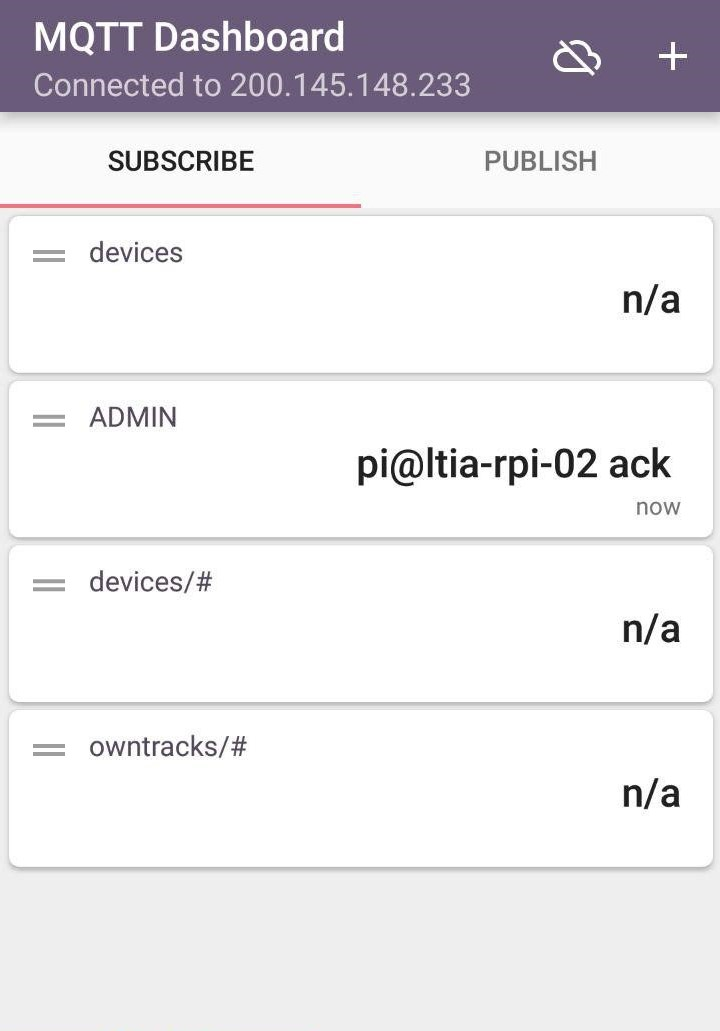
\includegraphics[width=1\textwidth]{052-gateway/mqtt/ad-home-ack.jpg}
		\legend{Fonte: Produzido pelo autor}
	\end{minipage}
\hfill
	\begin{minipage}{0.32\textwidth}
	\centering
		\caption{\label{fig-ad-admin-ack}MQTT Dashboard: Lista de mensagens no tópico}
		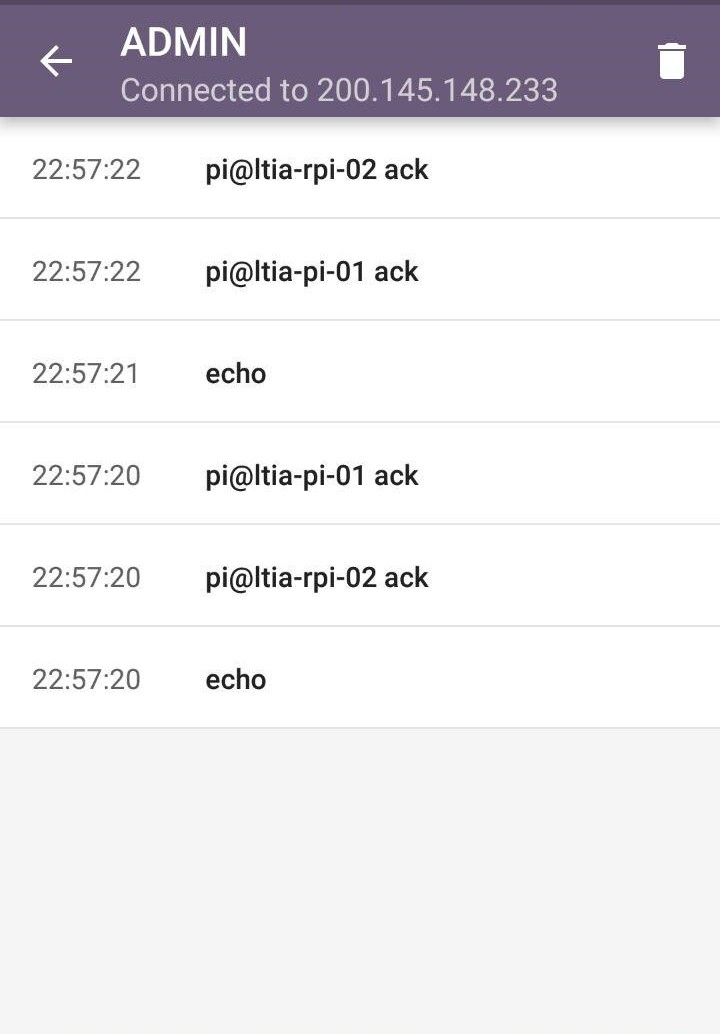
\includegraphics[width=1\textwidth]{052-gateway/mqtt/ad-admin-ack.jpg}
		\legend{Fonte: Produzido pelo autor}
	\end{minipage}
\end{figure}

\begin{figure}[htb]
	\centering
	\caption{\label{fig-mqttfx-stats}MQTT.fx: Estatísticas do \emph{Broker}}
	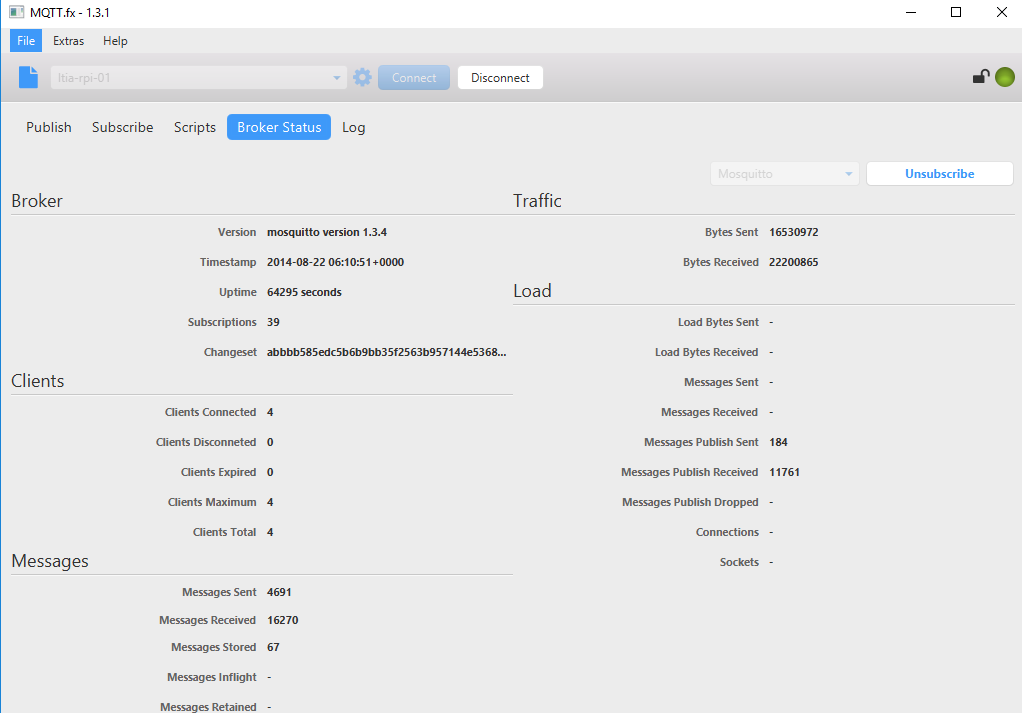
\includegraphics[width=1\textwidth]{052-gateway/mqtt/mqttfx-stats.png}
	\legend{Fonte: Produzido pelo autor}
\end{figure}

\begin{figure}[htb]
	\centering
	\caption{\label{fig-mqtt-spy-list}mqtt-spy: Listagem de dispositivos}
	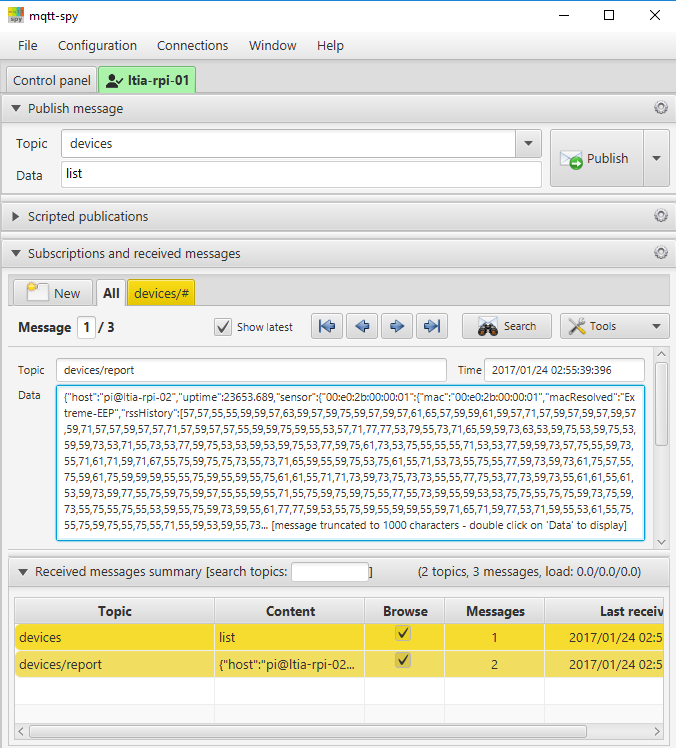
\includegraphics[width=1\textwidth]{052-gateway/mqtt/mqtt-spy-list.png}
	\legend{Fonte: Produzido pelo autor}
\end{figure}
